\let\negmedspace\undefined
\let\negthickspace\undefined
\documentclass[journal]{IEEEtran}
\usepackage[a5paper, margin=10mm, onecolumn]{geometry}
%\usepackage{lmodern} % Ensure lmodern is loaded for pdflatex
\usepackage{tfrupee} % Include tfrupee package

\setlength{\headheight}{1cm} % Set the height of the header box
\setlength{\headsep}{0mm}     % Set the distance between the header box and the top of the text

\usepackage{gvv-book}
\usepackage{gvv}
\usepackage{cite}
\usepackage{amsmath,amssymb,amsfonts,amsthm}
\usepackage{algorithmic}
\usepackage{graphicx}
\usepackage{textcomp}
\usepackage{xcolor}
\usepackage{txfonts}
\usepackage{listings}
\usepackage{enumitem}
\usepackage{mathtools}
\usepackage{gensymb}
\usepackage{comment}
\usepackage[breaklinks=true]{hyperref}
\usepackage{tkz-euclide} 
\usepackage{listings}
% \usepackage{gvv}                                        
\def\inputGnumericTable{}                                 
\usepackage[latin1]{inputenc}                                
\usepackage{color}                                            
\usepackage{array}                                            
\usepackage{longtable}                                       
\usepackage{calc}                                             
\usepackage{multirow}                                         
\usepackage{hhline}                                           
\usepackage{ifthen}                                           
\usepackage{lscape}
\begin{document}
\bibliographystyle{IEEEtran}
\title{5.3.36}
\author{EE25BTECH11002 - Achat Parth Kalpesh }
{\let\newpage\relax\maketitle}
\renewcommand{\thefigure}{\theenumi}
\renewcommand{\thetable}{\theenumi}
\setlength{\intextsep}{10pt} % Space between text and floats
\numberwithin{equation}{enumi}
\numberwithin{figure}{enumi}
\renewcommand{\thetable}{\theenumi}
\parindent 0px



\textbf{Question:}\\
Solve the system of equations
\begin{align}
    \frac{bx}{a} - \frac{ay}{b} + a + b = 0\\
    bx - ay + 2ab = 0 
\end{align}
\textbf{Solution:}\\
The above equation can be written as
\begin{align}
    \vec{n_1}^\top \vec{x} &= c_1 \\
    \vec{n_2}^\top \vec{x} &= c_2 \\
    \myvec{\vec{n_1}\\ \vec{n_2}}^\top \vec{x} &= \myvec{c_1\\c_2}
\end{align}
 \begin{align}   
     \vec{A} = \myvec{\vec{n_1}\\ \vec{n_2}}^\top \quad
     \vec{b} = \myvec{c_1\\c_2} 
\end{align}
    \begin{align}
    \vec{A} \vec{x} &= \vec{b}\\
    \myvec{\frac{b}{a} & -\frac{a}{b}\\ b & -a} \vec{x} &= \myvec{-a-b\\-2ab}
\end{align}
    \begin{align}
    \vec{A}^\top \vec{A} \neq \vec{I}
\end{align}
Performing row operations:
\begin{align}
\augvec{2}{1}{\frac{b}{a} & -\frac{a}{b} &-a-b\\ b & -a &-2ab}
&\xleftrightarrow[]{R_1 \leftarrow R_1-\frac{R_2}{b}}
\augvec{2}{1}{\frac{b-a}{a} & 0 & a-b\\ b & -a &-2ab}\\
\augvec{2}{1}{\frac{b-a}{a} & 0 & a-b \\ b & -a &-2ab}
&\xleftrightarrow[]{R_2 \leftarrow -\frac{ab}{b-a} R_1 + R_2}
\augvec{2}{1}{\frac{b-a}{a} & 0 & a-b \\ 0 & -a & -ab}\\
\augvec{2}{1}{\frac{b-a}{a} & 0 & a-b \\ 0 & -a & -ab}
&\xleftrightarrow[]{R_2 \leftarrow -\frac{R_2}{a}}
\augvec{2}{1}{\frac{b-a}{a} & 0 & a-b \\ 0 & 1 &  b}\\
\augvec{2}{1}{\frac{b-a}{a} & 0 & a-b \\ 0 & 1 & - b}
&\xleftrightarrow[]{R_1 \leftarrow \frac{a}{b-a} R_1}
\augvec{2}{1}{1 & 0 & -a \\ 0 & 1 &  b}
\end{align}
Thus,
\begin{align}
    \vec{x} = \myvec{-a\\b}
\end{align}

\begin{figure}[h]
    \centering
    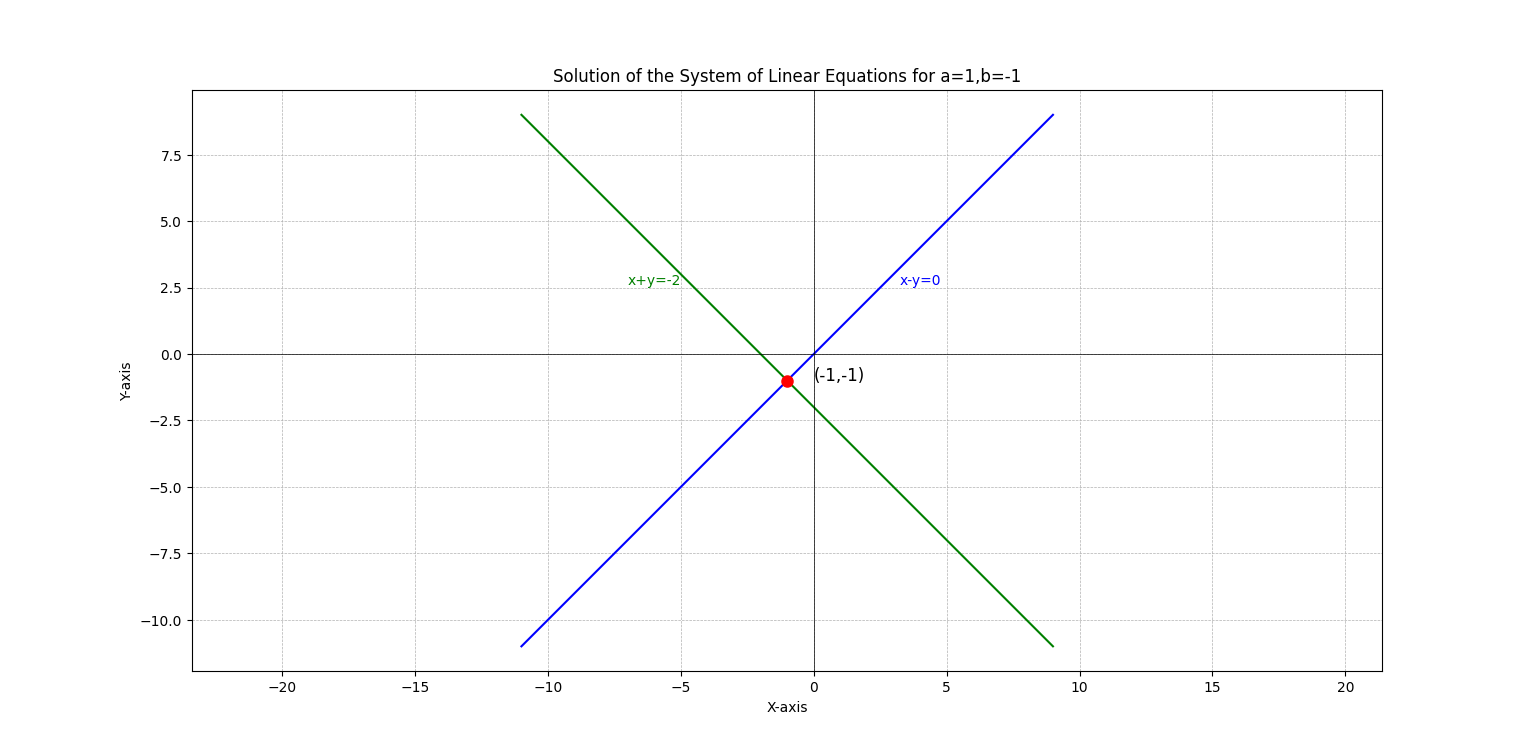
\includegraphics[width=\columnwidth]{figs/figure_py.png}
    \caption{Graph}
    \label{fig:fig}
 \end{figure}
\end{document}